\chapter{A model of constrained arbitrage in India}\label{ch:theory}
\chapterlead{One model in which every Indian limit to arbitrage is a parameter, written before the empirical work so that
the hypotheses are derived rather than fitted. This chapter states the results; the full version of the thesis gives the proofs
and numerical checks.}

\section{Set-up and the no-arbitrage band}
The basis is the gap between the futures price and its cost-of-carry value, $m=\ln F-\ln F^*$ with
$F^*=(S-\mathrm{PV}(D))e^{r(T-t)}$. Outside traders trade the stock and the future. Without arbitrage the basis equals
$u/\Phi$, where $u$ is the relative demand pressure toward futures and $\Phi$ measures the depth of the two markets. An
arbitrage sector holds $a$ units of the cash-and-carry trade (long stock, short future). Market clearing gives
\[ m=\frac{u-a}{\Phi}. \]
The sector chooses $a$ to maximise $am-\tfrac{\gamma}{2}a^2-c_+a^+-c_-a^-$, where $\gamma=\alpha\sigma^2$ reflects risk
aversion per unit of capital and the risk of the basis before convergence, $c_+$ is the cost of a cash-and-carry position
and $c_-$ the cost of a reverse position, which needs borrowed stock.

\emph{Result 1 (band).} Arbitrage starts only when the basis leaves $[-c_-,\,c_+]$. Inside, the basis moves one-for-one with
demand ($\partial m/\partial u=1/\Phi$); outside, arbitrage absorbs part of each shock (slope $\gamma/(\gamma\Phi+1)$). Figure~\ref{fig:modelband} draws this.

\begin{figure}[t]
\caption[The no-arbitrage band in the model]{Inside the band the basis follows demand one for one; outside it arbitrage absorbs part of each shock}\label{fig:modelband}
\exsub{Equilibrium basis against the demand pressure of outside traders, with illustrative costs $c_+=15$\bp\ and $c_-=60$\bp}
\centering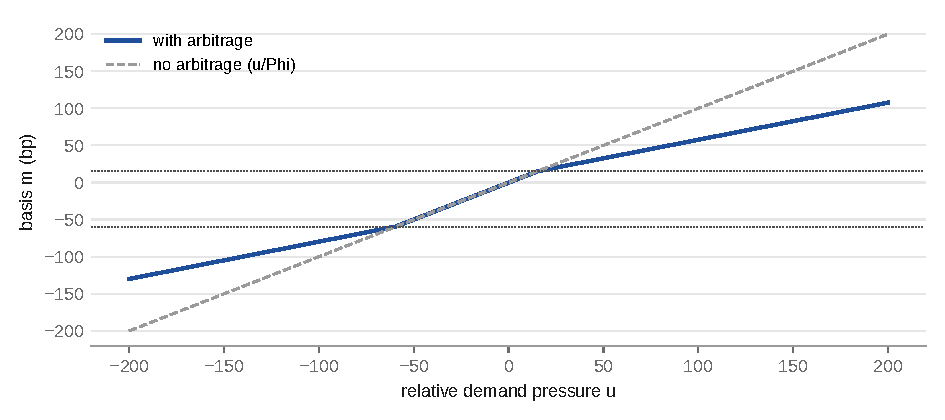
\includegraphics[width=0.92\linewidth]{model_band}
\exsource{Source: model of the full version of the thesis, Proposition C.1; illustrative parameters, not estimates.}
\end{figure}

\emph{Result 2 (comparative statics).} Costs set the edges one-for-one, so an STT increase should move the upper edge by
about the change in cost; capital and risk set how far the basis travels beyond an edge; the edges shrink as expiry
approaches; and because reverse arbitrage is costlier in India ($c_->c_+$), the band is centred below zero. With cheap,
tax-advantaged cash-and-carry capital whose required return is below the benchmark rate, even the upper edge can be negative.

\emph{Result 3 (inventory).} When the sector already holds $a_{t-1}$ and pays $c_u$ to unwind, it trades only when the basis
leaves $[\gamma a_{t-1}-c_u,\ \gamma a_{t-1}+c_+]$. Thresholds move with the size of the existing book. A threshold model with
fixed thresholds therefore estimates average edges, not costs; I confirmed this on data simulated from the model.

\section{The F\&O ban as a reduce-only rule}
In a ban, (B1) arbitrageurs may only reduce, $0\le a_t\le a_{t-1}$; and (B2) outside demand for \emph{new} futures exposure
cannot be executed: a share $\chi$ of it moves to the cash market (a trader who cannot buy the future buys the stock), and
the rest is withdrawn, while closing demand still trades.

\emph{Result 4 (one-sided correction).} A future that is too rich is no longer corrected, because nobody may open new
cash-and-carry positions: every increase in pressure passes through fully. A future that is too cheap is still corrected
by unwinding, at a floor $\gamma a_t-c_u$ that rises with the remaining book; the floor wears out as positions are
unwound, and an expiry inside the ban removes positions that cannot be rolled.


\emph{Result 5 (sign reversal).} In normal times new long demand raises the basis; in a ban the same demand lowers it,
because part of it moves to the stock.

\emph{Result 6 (level effect).} Relative to normal times, the ban raises the basis when pressure comes from closing trades
and lowers it when new speculative demand keeps arriving. Its sign is not fixed; the observable condition is the
composition of order flow.

\emph{Result 7 (trading).} If the rule binds contract by contract, every futures trade in a ban closes a long and a short,
so the change in open interest equals minus the volume; futures volume falls. Trades that offset across instruments
(allowed from October 2025) break the identity.

\section{Anticipation, hysteresis and identification}
\emph{Result 8 (anticipation).} If exit is costlier in a ban, the effective cost of opening cash-and-carry is
$c_++\pi(\omega)\ell$, where $\pi(\omega)$ is the chance that a position opened at utilisation $\omega$ meets a ban. The upper
edge rises smoothly as utilisation approaches 95\%; the jump at the trigger contains only the reduce-only effects. The model
does not sign a density test: arbitrageurs holding back thin the density below 95\%, speculators rushing in do the opposite.

\emph{Hysteresis.} Between 80\% and 95\% a stock may be in a ban or not; at equal utilisation the difference is the effect
of the reduce-only state against the anticipation state.

\emph{Result 9 (no instrument).} The MWPL enters the ban state, the anticipation term and entity limits. A change in the
MWPL moves the basis even without a ban, so it fails the exclusion restriction for an instrument of ban status;
denominator changes identify the effect of the whole position-limit regime.

\section{Short-sale constraints beyond the basis}
\emph{Result 10 (bad news in a ban).} If a share $\rho$ of informed selling runs through short futures, a ban lowers the
share of bad news impounded on the day from $k$ to $k(1-\rho)$, so drift after bad news rises; good news is unaffected.

\emph{Result 11 (Miller).} With dispersed valuations and costly shorting, prices reflect optimists; the overpricing with no
shorting is $(\sqrt{\delta}-\sqrt{Q/k})^2$, increasing in the dispersion $\delta$. Entry into the F\&O segment lowers the cost
of shorting, so it should lower overpricing and speed the incorporation of bad news (Diamond and Verrecchia, 1987); exit
should do the reverse.

\section{From results to hypotheses}
\begin{table}[t]
\caption[Hypotheses, their source and what would contradict them]{Every hypothesis comes from the model with the result that would contradict it}\label{tab:hyp}
\exsub{The first four form the primary family; the rest are secondary}
\small\begin{tabularx}{\textwidth}{@{}K{1.1cm}LL@{}}
\toprule
\thd{} & \thd{Prediction} & \thd{Contradicted if} \\
\midrule
H7 & In a ban, rich futures revert more slowly; cheap futures as fast or faster (Result 4) & No asymmetry, or the opposite \\ \rowrule
H8 & In a ban, futures volume falls and change in OI $\approx -$volume; cash activity rises (Result 7) & Futures activity unchanged \\ \rowrule
H3 & Band edges move with the STT, more for larger increases (Result 2) & Edges unrelated to cost changes \\ \rowrule
H6 & F\&O entry lowers price delay and bad-news drift; exit raises them (Result 11) & No change or the opposite \\ \rowrule
Level & The level effect follows the composition of order flow (Result 6) & Sign unrelated to composition \\ \rowrule
H9 & Upper tail rises smoothly toward 95\%; reforms act through utilisation (Results 8, 9) & Jump only at 95\% \\ \rowrule
H2 & Drift after bad news larger in a ban (Result 10) & Symmetric response \\ \rowrule
H1 & Wider bands where frictions are higher (Results 1 to 3) & No relation \\ \rowrule
H4 & Scarcer capital widens the band (Result 2) & No relation \\ \rowrule
H5 & Overpricing-side anomalies stronger where shorting is costly (Result 11) & Symmetric effects \\
\bottomrule
\end{tabularx}
\exsource{Source: model of the full version of the thesis; the frozen test plan of Appendix~\ref{app:plan}.}
\end{table}
H7, H8, H3 and H6 form the primary family, corrected jointly for multiple testing; the rest are secondary and reported
without adjustment.
